\section{Demi-droites graduées (4 points bonus)}

\begin{center}
	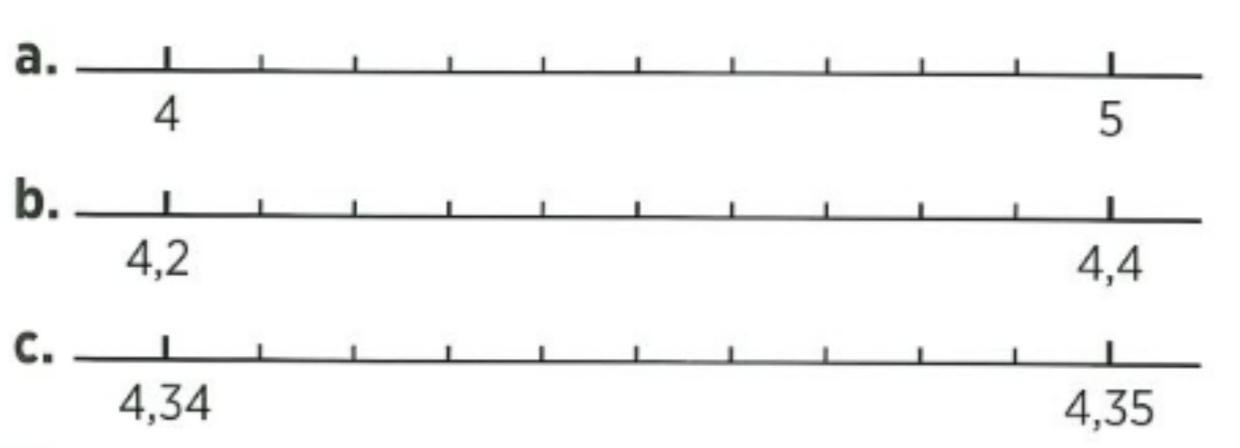
\includegraphics[scale=0.25]{img/axes}
\end{center}

\begin{questions}
	\question[1] Reproduire les trois demi-droites graduées ci-dessous:
	
	\question[3] En choisissant la demi-droite la mieux adaptée, placer les points suivants. On prolongera les demi-droites si besoin.
	
	\begin{multicols}{2}
		\begin{enumerate}
			\item $A\left( 4 + \dfrac{32}{100}\right)$
			\item $B\left(4 + \dfrac{3}{10} + \dfrac{4}{100} + \dfrac{2}{\num{1000}}\right)$
			\item $C(4 + \num{0.7})$
			\item $D\left(\dfrac{437}{100}\right)$
			\item $E\left(\dfrac{48}{10}\right)$
		\end{enumerate}
	\end{multicols}
\end{questions}